% Options for packages loaded elsewhere
\PassOptionsToPackage{unicode}{hyperref}
\PassOptionsToPackage{hyphens}{url}
%
\documentclass[
]{article}
\title{STOR 455 Class 6 R Notebook}
\author{}
\date{\vspace{-2.5em}}

\usepackage{amsmath,amssymb}
\usepackage{lmodern}
\usepackage{iftex}
\ifPDFTeX
  \usepackage[T1]{fontenc}
  \usepackage[utf8]{inputenc}
  \usepackage{textcomp} % provide euro and other symbols
\else % if luatex or xetex
  \usepackage{unicode-math}
  \defaultfontfeatures{Scale=MatchLowercase}
  \defaultfontfeatures[\rmfamily]{Ligatures=TeX,Scale=1}
\fi
% Use upquote if available, for straight quotes in verbatim environments
\IfFileExists{upquote.sty}{\usepackage{upquote}}{}
\IfFileExists{microtype.sty}{% use microtype if available
  \usepackage[]{microtype}
  \UseMicrotypeSet[protrusion]{basicmath} % disable protrusion for tt fonts
}{}
\makeatletter
\@ifundefined{KOMAClassName}{% if non-KOMA class
  \IfFileExists{parskip.sty}{%
    \usepackage{parskip}
  }{% else
    \setlength{\parindent}{0pt}
    \setlength{\parskip}{6pt plus 2pt minus 1pt}}
}{% if KOMA class
  \KOMAoptions{parskip=half}}
\makeatother
\usepackage{xcolor}
\IfFileExists{xurl.sty}{\usepackage{xurl}}{} % add URL line breaks if available
\IfFileExists{bookmark.sty}{\usepackage{bookmark}}{\usepackage{hyperref}}
\hypersetup{
  pdftitle={STOR 455 Class 6 R Notebook},
  hidelinks,
  pdfcreator={LaTeX via pandoc}}
\urlstyle{same} % disable monospaced font for URLs
\usepackage[margin=1in]{geometry}
\usepackage{color}
\usepackage{fancyvrb}
\newcommand{\VerbBar}{|}
\newcommand{\VERB}{\Verb[commandchars=\\\{\}]}
\DefineVerbatimEnvironment{Highlighting}{Verbatim}{commandchars=\\\{\}}
% Add ',fontsize=\small' for more characters per line
\usepackage{framed}
\definecolor{shadecolor}{RGB}{248,248,248}
\newenvironment{Shaded}{\begin{snugshade}}{\end{snugshade}}
\newcommand{\AlertTok}[1]{\textcolor[rgb]{0.94,0.16,0.16}{#1}}
\newcommand{\AnnotationTok}[1]{\textcolor[rgb]{0.56,0.35,0.01}{\textbf{\textit{#1}}}}
\newcommand{\AttributeTok}[1]{\textcolor[rgb]{0.77,0.63,0.00}{#1}}
\newcommand{\BaseNTok}[1]{\textcolor[rgb]{0.00,0.00,0.81}{#1}}
\newcommand{\BuiltInTok}[1]{#1}
\newcommand{\CharTok}[1]{\textcolor[rgb]{0.31,0.60,0.02}{#1}}
\newcommand{\CommentTok}[1]{\textcolor[rgb]{0.56,0.35,0.01}{\textit{#1}}}
\newcommand{\CommentVarTok}[1]{\textcolor[rgb]{0.56,0.35,0.01}{\textbf{\textit{#1}}}}
\newcommand{\ConstantTok}[1]{\textcolor[rgb]{0.00,0.00,0.00}{#1}}
\newcommand{\ControlFlowTok}[1]{\textcolor[rgb]{0.13,0.29,0.53}{\textbf{#1}}}
\newcommand{\DataTypeTok}[1]{\textcolor[rgb]{0.13,0.29,0.53}{#1}}
\newcommand{\DecValTok}[1]{\textcolor[rgb]{0.00,0.00,0.81}{#1}}
\newcommand{\DocumentationTok}[1]{\textcolor[rgb]{0.56,0.35,0.01}{\textbf{\textit{#1}}}}
\newcommand{\ErrorTok}[1]{\textcolor[rgb]{0.64,0.00,0.00}{\textbf{#1}}}
\newcommand{\ExtensionTok}[1]{#1}
\newcommand{\FloatTok}[1]{\textcolor[rgb]{0.00,0.00,0.81}{#1}}
\newcommand{\FunctionTok}[1]{\textcolor[rgb]{0.00,0.00,0.00}{#1}}
\newcommand{\ImportTok}[1]{#1}
\newcommand{\InformationTok}[1]{\textcolor[rgb]{0.56,0.35,0.01}{\textbf{\textit{#1}}}}
\newcommand{\KeywordTok}[1]{\textcolor[rgb]{0.13,0.29,0.53}{\textbf{#1}}}
\newcommand{\NormalTok}[1]{#1}
\newcommand{\OperatorTok}[1]{\textcolor[rgb]{0.81,0.36,0.00}{\textbf{#1}}}
\newcommand{\OtherTok}[1]{\textcolor[rgb]{0.56,0.35,0.01}{#1}}
\newcommand{\PreprocessorTok}[1]{\textcolor[rgb]{0.56,0.35,0.01}{\textit{#1}}}
\newcommand{\RegionMarkerTok}[1]{#1}
\newcommand{\SpecialCharTok}[1]{\textcolor[rgb]{0.00,0.00,0.00}{#1}}
\newcommand{\SpecialStringTok}[1]{\textcolor[rgb]{0.31,0.60,0.02}{#1}}
\newcommand{\StringTok}[1]{\textcolor[rgb]{0.31,0.60,0.02}{#1}}
\newcommand{\VariableTok}[1]{\textcolor[rgb]{0.00,0.00,0.00}{#1}}
\newcommand{\VerbatimStringTok}[1]{\textcolor[rgb]{0.31,0.60,0.02}{#1}}
\newcommand{\WarningTok}[1]{\textcolor[rgb]{0.56,0.35,0.01}{\textbf{\textit{#1}}}}
\usepackage{graphicx}
\makeatletter
\def\maxwidth{\ifdim\Gin@nat@width>\linewidth\linewidth\else\Gin@nat@width\fi}
\def\maxheight{\ifdim\Gin@nat@height>\textheight\textheight\else\Gin@nat@height\fi}
\makeatother
% Scale images if necessary, so that they will not overflow the page
% margins by default, and it is still possible to overwrite the defaults
% using explicit options in \includegraphics[width, height, ...]{}
\setkeys{Gin}{width=\maxwidth,height=\maxheight,keepaspectratio}
% Set default figure placement to htbp
\makeatletter
\def\fps@figure{htbp}
\makeatother
\setlength{\emergencystretch}{3em} % prevent overfull lines
\providecommand{\tightlist}{%
  \setlength{\itemsep}{0pt}\setlength{\parskip}{0pt}}
\setcounter{secnumdepth}{-\maxdimen} % remove section numbering
\ifLuaTeX
  \usepackage{selnolig}  % disable illegal ligatures
\fi

\begin{document}
\maketitle

\begin{Shaded}
\begin{Highlighting}[]
\CommentTok{\# message=FALSE, warning=FALSE suppress warnings and messages from appearing in knitted files}

\FunctionTok{library}\NormalTok{(readr)}
\FunctionTok{library}\NormalTok{(Stat2Data)}
\end{Highlighting}
\end{Shaded}

\textbf{Single Quantitative Predictor Model} Notation:\\
- Y = Response variable - X = Predictor variable

Assume (for now) that both Y and X are quantitative variables.

\textbf{Simple Linear Model} X = Single quantitative predictor Y =
Quantitative response

Find a line that best summarizes the trend in the data.

Y = Bo + B1X + E Response = intercept + Slope*Predictor + Random Error

\textbf{Simple Linear Model- Conditions} \textbf{Model:} 1.Linearity:
The means for Y vary as a linear function of X. \textbf{Error:} 2.Zero
Mean: The distribution of the errors is centered at zero. 3.Constant
variance: The variance for Y is the same at each X. (Homoscedasticity)
4.Independence: No relationships among errors. 5.Normality: Residuals
are normally distributed (sometimes) At each X, the Y's follow a normal
distribution.

\emph{Look at} What potent do these points have to influence our model?

\textbf{Types of ``Unusual'' Points in SLM} - Two Types -
\textbf{Outlier:} A data point that is far from the regression line.
--Points really above or below the regression line -- Doesn't always
have a lot of influence on the model -- Could be big enough that it has
influence, but mostly depends on the value of the predictor -- Data
points that are closer to the edges of the predictor value (high or low)
have a higher chance of having inlfuence in our model -
\textbf{Influential point:} A data point that has a large effect on the
regression fit. -- can come from many things

\textbf{Detecting Unusual Cases - Overview} 1. Compute residuals
``raw'', standardized, studentized 2. Plots of residuals (or std.
residuals) Boxplot, scatterplot, normal plot 3. Leverage Unusual values
for the predictors 4. Cook's distance Cases with large influence

\emph{This notebook covers the first two from above} - leverage = the
potiential for a certain value to have infleuence on the model - Cook's
distance combines a lot of the things to do some calculations for us

\textbf{Raw Residual} ei = yi - yhati \emph{How can we tell if a
residual is unusually large? } CONTEXT! Example: Y = GPA ei = 2.6 is
very large Y = SAT ei = 2.6 is very small

\textbf{Example: Men's Olympic Long Jump}

\begin{Shaded}
\begin{Highlighting}[]
\FunctionTok{data}\NormalTok{(}\StringTok{"LongJumpOlympics2016"}\NormalTok{)}
\FunctionTok{head}\NormalTok{(LongJumpOlympics2016)}
\end{Highlighting}
\end{Shaded}

\begin{verbatim}
##   Year  Gold
## 1 1900 7.185
## 2 1904 7.340
## 3 1906 7.200
## 4 1908 7.480
## 5 1912 7.600
## 6 1920 7.150
\end{verbatim}

\begin{Shaded}
\begin{Highlighting}[]
\FunctionTok{plot}\NormalTok{(Gold}\SpecialCharTok{\textasciitilde{}}\NormalTok{Year, }\AttributeTok{data=}\NormalTok{LongJumpOlympics2016) }\CommentTok{\# Predict longjump distance by year }
\NormalTok{GoldModel }\OtherTok{=} \FunctionTok{lm}\NormalTok{(Gold}\SpecialCharTok{\textasciitilde{}}\NormalTok{Year, }\AttributeTok{data=}\NormalTok{LongJumpOlympics2016)}
\FunctionTok{abline}\NormalTok{(GoldModel) }\CommentTok{\# Draw the line we made onto the plot}
\end{Highlighting}
\end{Shaded}

\includegraphics{STOR-455---Class-6---R-Notebook_files/figure-latex/unnamed-chunk-3-1.pdf}

\begin{Shaded}
\begin{Highlighting}[]
\FunctionTok{plot}\NormalTok{(GoldModel, }\DecValTok{1}\SpecialCharTok{:}\DecValTok{2}\NormalTok{) }\CommentTok{\# To see the residual models, we see that there is one really big outlier}
\end{Highlighting}
\end{Shaded}

\includegraphics{STOR-455---Class-6---R-Notebook_files/figure-latex/unnamed-chunk-3-2.pdf}
\includegraphics{STOR-455---Class-6---R-Notebook_files/figure-latex/unnamed-chunk-3-3.pdf}

\begin{Shaded}
\begin{Highlighting}[]
\CommentTok{\# Linearity looks like an issue because of the fitted plot.  The red line goes down; the prediction curves }
\CommentTok{\# Point 16 is our outlier }
\CommentTok{\# R tells us which row this is because it looks like an ourlier to R }
\CommentTok{\# Looking at the normal QQ Plot, normal might be an issue }
\CommentTok{\# Constant variance doesn\textquotesingle{}t appear to be an issue }
\FunctionTok{summary}\NormalTok{(GoldModel)}
\end{Highlighting}
\end{Shaded}

\begin{verbatim}
## 
## Call:
## lm(formula = Gold ~ Year, data = LongJumpOlympics2016)
## 
## Residuals:
##      Min       1Q   Median       3Q      Max 
## -0.39610 -0.15495 -0.00137  0.11606  0.75349 
## 
## Coefficients:
##               Estimate Std. Error t value Pr(>|t|)    
## (Intercept) -16.470194   2.666282  -6.177 1.56e-06 ***
## Year          0.012508   0.001361   9.191 1.19e-09 ***
## ---
## Signif. codes:  0 '***' 0.001 '**' 0.01 '*' 0.05 '.' 0.1 ' ' 1
## 
## Residual standard error: 0.2595 on 26 degrees of freedom
## Multiple R-squared:  0.7646, Adjusted R-squared:  0.7556 
## F-statistic: 84.47 on 1 and 26 DF,  p-value: 1.192e-09
\end{verbatim}

\begin{Shaded}
\begin{Highlighting}[]
\CommentTok{\# Look at estimate of the year: For every 1 year increase than that\textquotesingle{}s how many meters we think the winning long distance jump is going to increase as well }
\CommentTok{\# Every 4 years it looks like its increasing by 5 cms}
\end{Highlighting}
\end{Shaded}

\textbf{What if we wanted to see what the data looked like without the
outlier?}

\begin{Shaded}
\begin{Highlighting}[]
\FunctionTok{boxplot}\NormalTok{(GoldModel}\SpecialCharTok{$}\NormalTok{residuals)}
\end{Highlighting}
\end{Shaded}

\includegraphics{STOR-455---Class-6---R-Notebook_files/figure-latex/unnamed-chunk-4-1.pdf}

\begin{Shaded}
\begin{Highlighting}[]
\CommentTok{\# Outliers are more than 1.5 IQR’s beyond the Quartiles}
\CommentTok{\# Will give idea of how different that one value is from the others }

\CommentTok{\# Wee see there is an outlier, but how much of an outlier is this? }
\CommentTok{\# LOOK AT STANDARDIZED VALUES OF RESIDUALS INSTEAD}

\FunctionTok{max}\NormalTok{(GoldModel}\SpecialCharTok{$}\NormalTok{residuals)}
\end{Highlighting}
\end{Shaded}

\begin{verbatim}
## [1] 0.7534932
\end{verbatim}

\begin{Shaded}
\begin{Highlighting}[]
\FunctionTok{which.max}\NormalTok{(GoldModel}\SpecialCharTok{$}\NormalTok{residuals)}
\end{Highlighting}
\end{Shaded}

\begin{verbatim}
## 16 
## 16
\end{verbatim}

\textbf{Standardized Residuals} - HOW TO TELL HOW MUCH OF AN OUTLIER
THIS IS - ROughly equal to the acutal - predicted/stdeve; basically a
zscore, but not exactly

\begin{itemize}
\item
  Fact: If X has mean mu and std. dev, then (𝑋−𝜇)/𝜎 has mean 0 and std.
  dev.=1.
\item
  For residuals: mean=0 and std. dev. of errors
\item
  Standardized Residuals about equals (yi - yhat)/stad dev of the
  population errors
\item
  Look for values beyond +/-2 (mild) or beyond +/-3
\item
  Once you have fit mymodel=lm(Y\textasciitilde X)
\item
  Use: rstandard(mymodel)
\end{itemize}

\emph{notes} - It will give us a thing centered at zero +/- unites; and
that's how many std they are away from teh average - THink about this
as: - Once you are +/- 2 std away and its normally dist, then you're in
teh outer 5\% of the data, so that's starting to eb an outlier - IF
you're +/-3 away, then you're into the .05 of the data and outliers, so
it's pretty extreme

\emph{Below} - If we look at the standaized residual, it's 2.96. so it's
2.96 std above the line, which is an outlier

\begin{Shaded}
\begin{Highlighting}[]
\FunctionTok{rstandard}\NormalTok{(GoldModel) }\CommentTok{\# Put the model in }
\end{Highlighting}
\end{Shaded}

\begin{verbatim}
##           1           2           3           4           5           6 
## -0.45846037 -0.02447194 -0.69927805  0.34245659  0.62395356 -1.58872766 
##           7           8           9          10          11          12 
## -0.60354515  0.33349306 -0.22282237  1.24041457 -0.28038843 -1.47783119 
##          13          14          15          16          17          18 
## -0.65303672  0.28865616 -0.10391829  2.96025507  0.17095826  0.40756162 
##          19          20          21          22          23          24 
##  0.96124413  0.76569814  1.28443310  0.89029407  0.01303494  0.01295953 
##          25          26          27          28 
## -0.02754601 -1.24791995 -1.58338033 -1.51206192
\end{verbatim}

\begin{Shaded}
\begin{Highlighting}[]
\CommentTok{\# Will show standardized residuals }
\CommentTok{\# Taht\textquotesingle{}s great when we have a small dataset, but if its not small, then don\textquotesingle{}t use the above code }

\FunctionTok{which.max}\NormalTok{(GoldModel}\SpecialCharTok{$}\NormalTok{residuals)}
\end{Highlighting}
\end{Shaded}

\begin{verbatim}
## 16 
## 16
\end{verbatim}

\begin{Shaded}
\begin{Highlighting}[]
\FunctionTok{rstandard}\NormalTok{(GoldModel)[}\DecValTok{16}\NormalTok{] }\CommentTok{\# This will target the key point we ar elooking at }
\end{Highlighting}
\end{Shaded}

\begin{verbatim}
##       16 
## 2.960255
\end{verbatim}

\textbf{We now know it's an outlier, BUT WE DONT KNOW IF IT HAS ANY
INFLUENCE ON TEH MODEL YET} - Can plot the rstand of the residuals by
the fitted values - The plot is going to look identical to the others,
other htan the axies, so but it's a different measure of scale - How
much infleunce is that really having?

\begin{Shaded}
\begin{Highlighting}[]
\FunctionTok{plot}\NormalTok{(}\FunctionTok{rstandard}\NormalTok{(GoldModel)}\SpecialCharTok{\textasciitilde{}}\NormalTok{GoldModel}\SpecialCharTok{$}\NormalTok{fitted.values)}
\FunctionTok{abline}\NormalTok{(}\DecValTok{0}\NormalTok{,}\DecValTok{0}\NormalTok{)}
\end{Highlighting}
\end{Shaded}

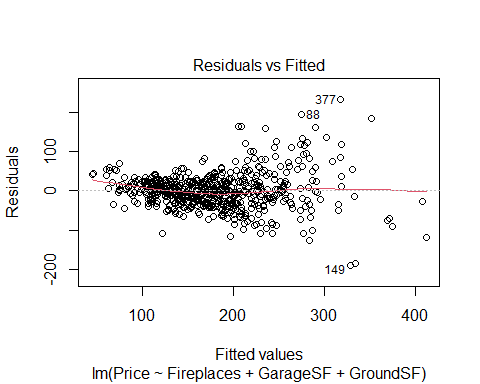
\includegraphics{STOR-455---Class-6---R-Notebook_files/figure-latex/unnamed-chunk-6-1.pdf}
\textbf{THING ABOUT THE STUDNTIZED RESIDUALS TO SEE HOW MUCH INFLUENCE
SOMETHING HAS} - Standard = Outliers - Student = Influence (uses a
different standard deviation)

\textbf{Studentized Residual} - Takes the single data out of the
dataset, make a new regression line and get a new std of resid and
seeing how far away the new line is from the outlier point in terms of
the new standard residuals - If we take out an oulter, the std of the
residuals is going to go down because we are removing an extreme case,
so now its going to take more std to get to the outlier, and its going
to give us a value that is bigger - When we see a studentized residual
that is larger thant the stadnard residual, then it tells us that by
removing this point, we are reallying changing the varibaility of the
model and condenseing it more. - uses a different standard deviation
than standariza

\begin{itemize}
\item
  \textbf{Concern:} An unusual value may exert great influence on the
  fit
\item
  Its residual might be underestimated because the model ``moves'' a lot
  to fit it and/or
\item
  The standard error of regression may be inflated due to the outlier
  error
\item
  \textbf{Studentize:} Fit the model without that case, then find new
  𝑦−𝑦hat and 𝜎\_𝜀 (of the population) to standardize. (R does this for
  every point)
\end{itemize}

\textbf{Influence} The effect of a single data point on the regression
line depends on: - how well it matches the ``trend'' of the rest of the
points - how ``unusual'' is its predictor value

\begin{Shaded}
\begin{Highlighting}[]
\FunctionTok{plot}\NormalTok{(}\FunctionTok{rstudent}\NormalTok{(GoldModel)}\SpecialCharTok{\textasciitilde{}}\NormalTok{GoldModel}\SpecialCharTok{$}\NormalTok{fitted.values)}
\FunctionTok{abline}\NormalTok{(}\DecValTok{0}\NormalTok{,}\DecValTok{0}\NormalTok{)}
\end{Highlighting}
\end{Shaded}

\includegraphics{STOR-455---Class-6---R-Notebook_files/figure-latex/unnamed-chunk-7-1.pdf}

\begin{Shaded}
\begin{Highlighting}[]
\FunctionTok{rstudent}\NormalTok{(GoldModel)[}\DecValTok{16}\NormalTok{]}
\end{Highlighting}
\end{Shaded}

\begin{verbatim}
##       16 
## 3.565083
\end{verbatim}

\begin{Shaded}
\begin{Highlighting}[]
\CommentTok{\# When we took the outlier from teh thing, its more away, which is bigger }
\CommentTok{\# There is some kind of influence here, but is it really noticable influence? }
\end{Highlighting}
\end{Shaded}

\begin{Shaded}
\begin{Highlighting}[]
\CommentTok{\# plot(IceModel3) \# From the previous notes }

\CommentTok{\# max(rstandard(IceModel3))}
\CommentTok{\# max(rstudent(IceModel3))}
\CommentTok{\# When we look at the values, themore different they are the mode influence they have in the model }
\CommentTok{\# The more close they are, then they have less influence on the model }
\CommentTok{\# No real bounds on what is a big or little influence on set number ot look at }
\end{Highlighting}
\end{Shaded}

\textbf{Dataset: PalmBeach} - County vote counts in Florida (n=67) for
George Bush and Pat Buchanan in 2000. - Model: Use Bush votes to predict
Buchanan votes.

\begin{Shaded}
\begin{Highlighting}[]
\FunctionTok{data}\NormalTok{(PalmBeach)}
\FunctionTok{head}\NormalTok{(PalmBeach)}
\end{Highlighting}
\end{Shaded}

\begin{verbatim}
##     County Buchanan   Bush
## 1  ALACHUA      262  34062
## 2    BAKER       73   5610
## 3      BAY      248  38637
## 4 BRADFORD       65   5413
## 5  BREVARD      570 115185
## 6  BROWARD      789 177279
\end{verbatim}

\begin{Shaded}
\begin{Highlighting}[]
\NormalTok{ElectionModel }\OtherTok{=} \FunctionTok{lm}\NormalTok{(Buchanan}\SpecialCharTok{\textasciitilde{}}\NormalTok{Bush, }\AttributeTok{data=}\NormalTok{PalmBeach)}
\CommentTok{\# Bush = republican }
\CommentTok{\# Buchana {-} the other person }

\FunctionTok{plot}\NormalTok{(Buchanan}\SpecialCharTok{\textasciitilde{}}\NormalTok{Bush, }\AttributeTok{data=}\NormalTok{PalmBeach) }\CommentTok{\# Look at the residuals and check the conditions }
\FunctionTok{abline}\NormalTok{(ElectionModel)}
\end{Highlighting}
\end{Shaded}

\includegraphics{STOR-455---Class-6---R-Notebook_files/figure-latex/unnamed-chunk-9-1.pdf}
\textbf{Example: Palm Beach Butterfly Ballot} - Palm Beach is the
outlier

\begin{Shaded}
\begin{Highlighting}[]
\FunctionTok{plot}\NormalTok{(ElectionModel, }\DecValTok{1}\SpecialCharTok{:}\DecValTok{2}\NormalTok{)}
\end{Highlighting}
\end{Shaded}

\includegraphics{STOR-455---Class-6---R-Notebook_files/figure-latex/unnamed-chunk-10-1.pdf}
\includegraphics{STOR-455---Class-6---R-Notebook_files/figure-latex/unnamed-chunk-10-2.pdf}

\begin{Shaded}
\begin{Highlighting}[]
\FunctionTok{plot}\NormalTok{(}\FunctionTok{rstudent}\NormalTok{(ElectionModel)}\SpecialCharTok{\textasciitilde{}}\NormalTok{ElectionModel}\SpecialCharTok{$}\NormalTok{fitted.values)}
\FunctionTok{abline}\NormalTok{(}\DecValTok{0}\NormalTok{,}\DecValTok{0}\NormalTok{)}
\end{Highlighting}
\end{Shaded}

\includegraphics{STOR-455---Class-6---R-Notebook_files/figure-latex/unnamed-chunk-10-3.pdf}

\begin{Shaded}
\begin{Highlighting}[]
\FunctionTok{plot}\NormalTok{(}\FunctionTok{rstandard}\NormalTok{(ElectionModel)}\SpecialCharTok{\textasciitilde{}}\NormalTok{ElectionModel}\SpecialCharTok{$}\NormalTok{fitted.values)}
\FunctionTok{abline}\NormalTok{(}\DecValTok{0}\NormalTok{,}\DecValTok{0}\NormalTok{)}
\end{Highlighting}
\end{Shaded}

\includegraphics{STOR-455---Class-6---R-Notebook_files/figure-latex/unnamed-chunk-10-4.pdf}

\begin{Shaded}
\begin{Highlighting}[]
\FunctionTok{boxplot}\NormalTok{(ElectionModel}\SpecialCharTok{$}\NormalTok{residuals, }\AttributeTok{horizontal=}\ConstantTok{TRUE}\NormalTok{) }\CommentTok{\# Look at the outliers, there looks like ther eare a lot of outliers, but it\textquotesingle{}s okay we are only looking at one of them }
\end{Highlighting}
\end{Shaded}

\includegraphics{STOR-455---Class-6---R-Notebook_files/figure-latex/unnamed-chunk-10-5.pdf}

\textbf{What to do with an extreme residual?} - Try a transformation
(Loging works really well, log(Data)) - Redo the analysis with the point
omitted

\emph{Below, we redo with the point omitted}

\begin{Shaded}
\begin{Highlighting}[]
\NormalTok{newdata }\OtherTok{=} \FunctionTok{subset}\NormalTok{(PalmBeach, County}\SpecialCharTok{!=}\StringTok{"PALM BEACH"}\NormalTok{)}

\NormalTok{ElectionModel\_noPB }\OtherTok{=} \FunctionTok{lm}\NormalTok{(Buchanan}\SpecialCharTok{\textasciitilde{}}\NormalTok{Bush, }\AttributeTok{data=}\NormalTok{newdata)}

\FunctionTok{summary}\NormalTok{(ElectionModel)}
\end{Highlighting}
\end{Shaded}

\begin{verbatim}
## 
## Call:
## lm(formula = Buchanan ~ Bush, data = PalmBeach)
## 
## Residuals:
##     Min      1Q  Median      3Q     Max 
## -907.50  -46.10  -29.19   12.26 2610.19 
## 
## Coefficients:
##              Estimate Std. Error t value Pr(>|t|)    
## (Intercept) 4.529e+01  5.448e+01   0.831    0.409    
## Bush        4.917e-03  7.644e-04   6.432 1.73e-08 ***
## ---
## Signif. codes:  0 '***' 0.001 '**' 0.01 '*' 0.05 '.' 0.1 ' ' 1
## 
## Residual standard error: 353.9 on 65 degrees of freedom
## Multiple R-squared:  0.3889, Adjusted R-squared:  0.3795 
## F-statistic: 41.37 on 1 and 65 DF,  p-value: 1.727e-08
\end{verbatim}

\begin{Shaded}
\begin{Highlighting}[]
\FunctionTok{summary}\NormalTok{(ElectionModel\_noPB)}
\end{Highlighting}
\end{Shaded}

\begin{verbatim}
## 
## Call:
## lm(formula = Buchanan ~ Bush, data = newdata)
## 
## Residuals:
##     Min      1Q  Median      3Q     Max 
## -512.43  -47.97  -17.09   41.78  305.45 
## 
## Coefficients:
##              Estimate Std. Error t value Pr(>|t|)    
## (Intercept) 6.557e+01  1.733e+01   3.784 0.000343 ***
## Bush        3.482e-03  2.501e-04  13.923  < 2e-16 ***
## ---
## Signif. codes:  0 '***' 0.001 '**' 0.01 '*' 0.05 '.' 0.1 ' ' 1
## 
## Residual standard error: 112.5 on 64 degrees of freedom
## Multiple R-squared:  0.7518, Adjusted R-squared:  0.7479 
## F-statistic: 193.8 on 1 and 64 DF,  p-value: < 2.2e-16
\end{verbatim}

\begin{Shaded}
\begin{Highlighting}[]
\CommentTok{\# Compare teh summary of old vs new model }
\CommentTok{\# We see that the new model residuals std error is really high; it s std value }
\CommentTok{\# The origanl value is a lot smaller for std}
\end{Highlighting}
\end{Shaded}

\textbf{Model with/without Palm Beach} - If compare the rstudent and
rstandard of the with palm beach, we see that there is a really big jump
between tehse numbers; tells us we have a value that is taking the whole
regression and dragging it - So all our other predictiosn are going to
be higher becuase of this vlaue

\begin{itemize}
\tightlist
\item
  If we look at the intercept and slope
\item
  the slope is more dramatic when we take out the point, with the
  intercept goes down
\item
  the residual standarad errors are very different between teh two
\item
  the linearirity is really good without the palm beach
\item
  the normal residuals look pretty bad when you take out palm beach
\end{itemize}

\begin{Shaded}
\begin{Highlighting}[]
\FunctionTok{plot}\NormalTok{(ElectionModel\_noPB, }\DecValTok{1}\SpecialCharTok{:}\DecValTok{2}\NormalTok{)}
\end{Highlighting}
\end{Shaded}

\includegraphics{STOR-455---Class-6---R-Notebook_files/figure-latex/unnamed-chunk-12-1.pdf}
\includegraphics{STOR-455---Class-6---R-Notebook_files/figure-latex/unnamed-chunk-12-2.pdf}

\begin{Shaded}
\begin{Highlighting}[]
\FunctionTok{plot}\NormalTok{(}\FunctionTok{rstudent}\NormalTok{(ElectionModel\_noPB)}\SpecialCharTok{\textasciitilde{}}\NormalTok{ElectionModel\_noPB}\SpecialCharTok{$}\NormalTok{fitted.values)}
\FunctionTok{abline}\NormalTok{(}\DecValTok{0}\NormalTok{,}\DecValTok{0}\NormalTok{)}
\end{Highlighting}
\end{Shaded}

\includegraphics{STOR-455---Class-6---R-Notebook_files/figure-latex/unnamed-chunk-12-3.pdf}

\begin{Shaded}
\begin{Highlighting}[]
\FunctionTok{plot}\NormalTok{(}\FunctionTok{rstandard}\NormalTok{(ElectionModel\_noPB)}\SpecialCharTok{\textasciitilde{}}\NormalTok{ElectionModel\_noPB}\SpecialCharTok{$}\NormalTok{fitted.values)}
\FunctionTok{abline}\NormalTok{(}\DecValTok{0}\NormalTok{,}\DecValTok{0}\NormalTok{)}
\end{Highlighting}
\end{Shaded}

\includegraphics{STOR-455---Class-6---R-Notebook_files/figure-latex/unnamed-chunk-12-4.pdf}

\begin{Shaded}
\begin{Highlighting}[]
\FunctionTok{boxplot}\NormalTok{(ElectionModel\_noPB}\SpecialCharTok{$}\NormalTok{residuals, }\AttributeTok{horizontal=}\ConstantTok{TRUE}\NormalTok{)}
\end{Highlighting}
\end{Shaded}

\includegraphics{STOR-455---Class-6---R-Notebook_files/figure-latex/unnamed-chunk-12-5.pdf}

\textbf{BE careful with the student and standard} - look at how differen
tbetween student and standard, you cna't just know based on the one
value

\end{document}
